%\subsection{Beispiel HS19, Residuensatz}

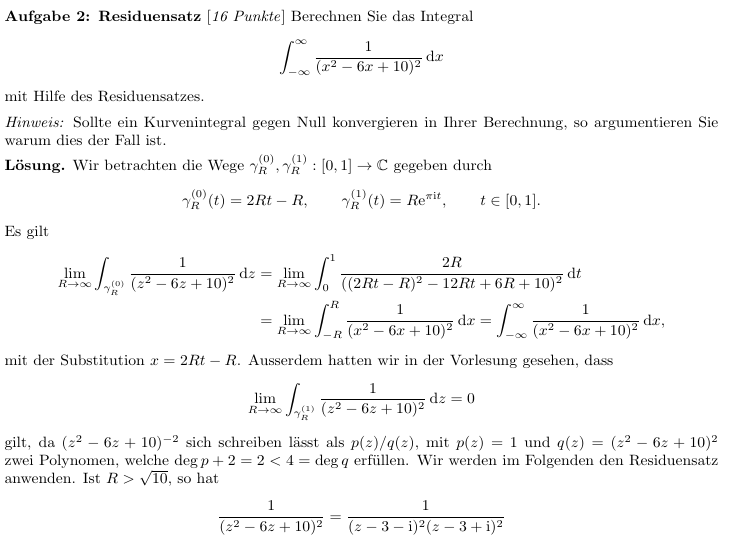
\includegraphics[width=1\textwidth]{images/img_koma/example_1.1_hs19.png}
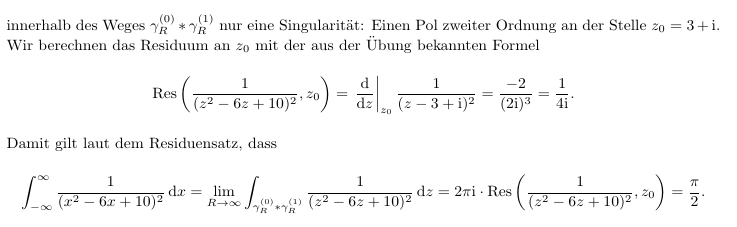
\includegraphics[width=1\textwidth]{images/img_koma/example_1.2_hs19.png}

%\subsection{Beispiel HS19, Laplace-Transform}
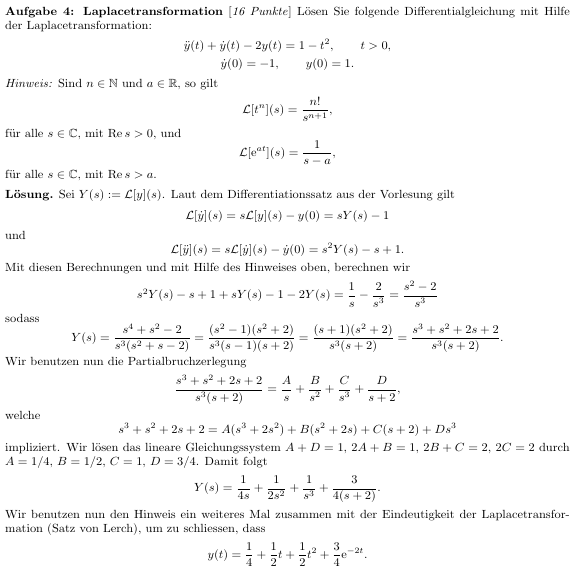
\includegraphics[width=1\textwidth]{images/img_koma/example_1.3_hs19.png}

%\subsection{Beispiel HS19, Fourierreihe}
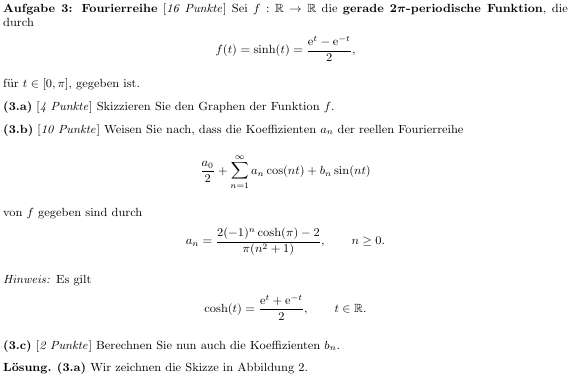
\includegraphics[width=1\textwidth]{images/img_koma/example_1.4.1_hs19.png}
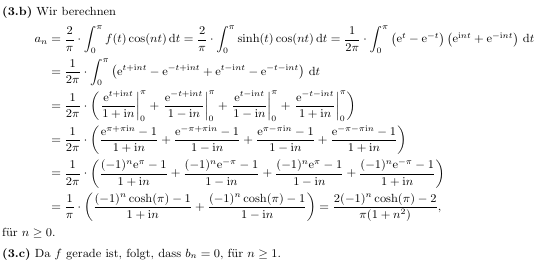
\includegraphics[width=1\textwidth]{images/img_koma/example_1.4.2_hs19.png}
%\footnotesize{Beispiel HS19, Fourierreihe}

%\subsection{Beispiel FS18, Residuensatz}
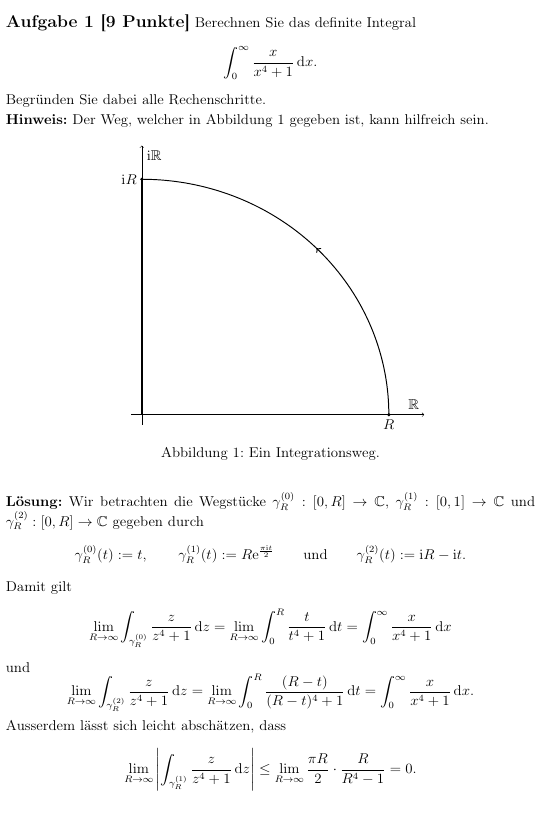
\includegraphics[width=1\textwidth]{images/img_koma/example_1.5.1_fs18.png}
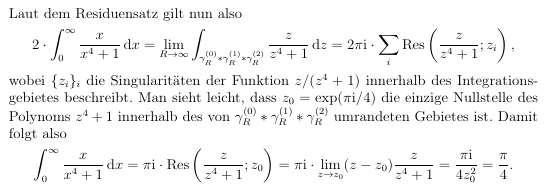
\includegraphics[width=1\textwidth]{images/img_koma/example_1.5.2_fs18.png}


%\subsection{Beispiel FS18, Residuensatz}
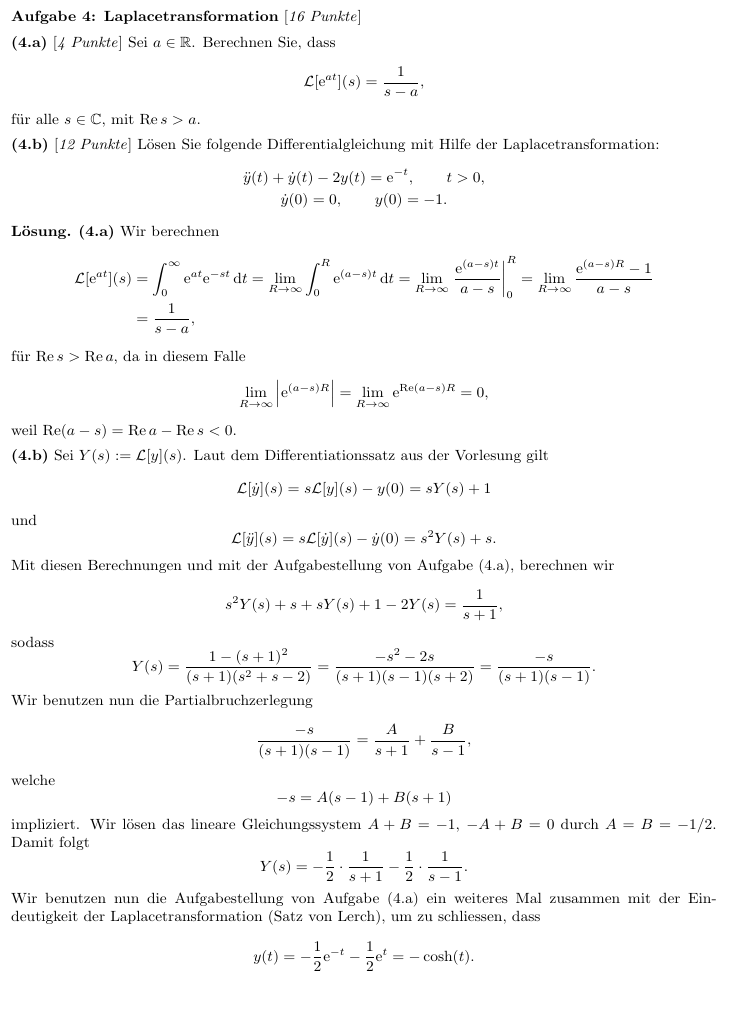
\includegraphics[width=1\textwidth]{images/img_koma/example_1.6_fs19.png}


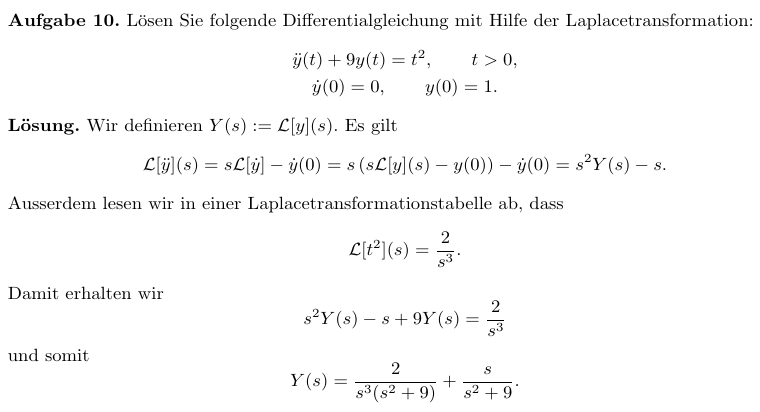
\includegraphics[width=1\textwidth]{images/img_koma/lapl1.png}
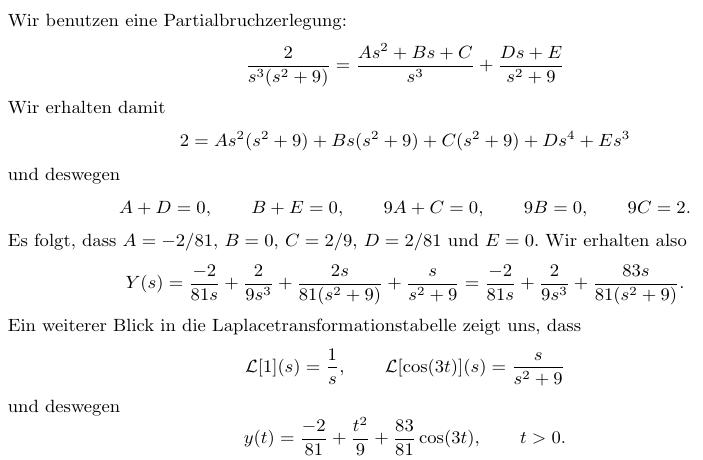
\includegraphics[width=1\textwidth]{images/img_koma/lapl2.png}
Residue\\
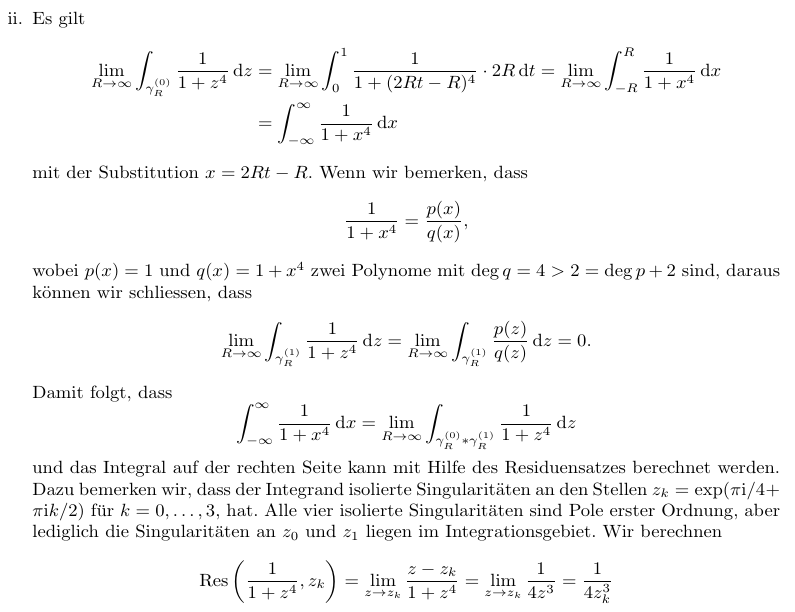
\includegraphics[width=1\textwidth]{images/img_koma/residue1.png}
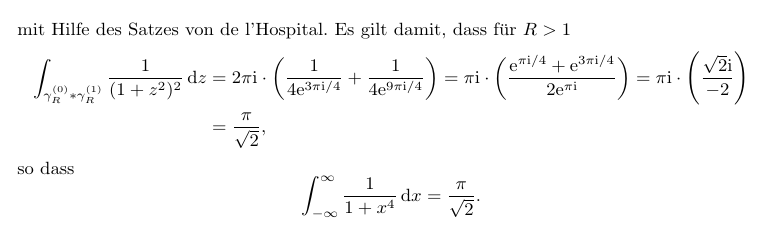
\includegraphics[width=1\textwidth]{images/img_koma/residue2.png}
